\documentclass[12pt, a4paper]{report}

% Packages :

\usepackage[french]{babel}
\usepackage[utf8]{inputenc}
\usepackage[T1]{fontenc}
\usepackage[pdftex, pdfauthor={Bacomathiques}]{hyperref}
\usepackage{sectsty}
\usepackage[explicit]{titlesec}
\usepackage{xcolor}
\usepackage{amsmath}
\usepackage{amssymb}
\usepackage{amsthm}
\usepackage{fourier}
\usepackage{titlesec}
\usepackage{fancyhdr}
\usepackage{catchfilebetweentags}
\usepackage[french, capitalise, noabbrev]{cleveref}
\usepackage[fit, breakall]{truncate}
\usepackage[margin=3cm]{geometry}
\usepackage{tocloft}
\usepackage{tikz}
\usepackage{tocloft}
\usepackage{microtype}
\usepackage{listings}
\usepackage{tabularx}
\usepackage{calc}
\usepackage[export]{adjustbox}
\usepackage[most]{tcolorbox}
\usepackage{standalone}
\usepackage{xlop}
\usepackage{etoolbox}
\usepackage{environ}

\usetikzlibrary{arrows.meta}
\usetikzlibrary{trees}

% Paramètres :

\author{Bacomathiques}
\definecolor{graphe}{HTML}{93c9ff}
\setcounter{MaxMatrixCols}{12}
\setlength{\parindent}{0pt}
\setlength{\fboxsep}{0pt}
%\pdfsuppresswarningpagegroup=1

% Code :

\lstdefinestyle{style}{
	backgroundcolor=\color{white},
	commentstyle=\em\color[HTML]{999988},
	keywordstyle=\bfseries,
	identifierstyle=\normalfont,
	stringstyle=\color[rgb]{0.87, 0.07, 0.27},
	basicstyle=\ttfamily\color{black},
	breakatwhitespace=false,
	breaklines=true,
	captionpos=b,
	keepspaces=true,
	numbers=left,
	numbersep=5pt,
	showspaces=false,
	showstringspaces=false,
	showtabs=false,
	tabsize=2,
	numbers=none
}

\lstset{style=style}
\lstset{
	literate=
	{á}{{\'a}}1
	{à}{{\`a}}1
	{ã}{{\~a}}1
	{é}{{\'e}}1
	{ê}{{\^e}}1
	{í}{{\'i}}1
	{ó}{{\'o}}1
	{õ}{{\~o}}1
	{ú}{{\'u}}1
	{ü}{{\"u}}1
	{ç}{{\c{c}}}1
}

\lstset{
	framextopmargin=10pt,
	framexrightmargin=10pt,
	framexbottommargin=10pt,
	framexleftmargin=10pt,
	xleftmargin=10pt,
	xrightmargin=10pt,
}

% Couleurs :

\definecolor{title}{HTML}{912c21}
\definecolor{section}{HTML}{1c567d}
\definecolor{subsection}{HTML}{2980b9}

\definecolor{rule}{HTML}{c4c4c4}

\definecolor{formula}{HTML}{ebf3fb}
\definecolor{formula-left}{HTML}{3583d6}

\definecolor{tip}{HTML}{dcf3d8}
\definecolor{tip-left}{HTML}{26a65b}

\definecolor{demonstration}{HTML}{fff8de}
\definecolor{demonstration-left}{HTML}{f1c40f}

\definecolor{exercise}{HTML}{e0f2f1}
\definecolor{exercise-left}{HTML}{009688}

\definecolor{correction}{HTML}{e0f7fa}
\definecolor{correction-left}{HTML}{00bcd4}

\definecolor{toc}{HTML}{fceae9}
\definecolor{toc-left}{HTML}{e74c3c}
\definecolor{toc-dark}{HTML}{87281f}

% Titres :

\renewcommand{\thesection}{\Roman{section} - }
\renewcommand{\thesubsection}{\arabic{subsection}. }

\newcommand{\sectionstyle}{\normalfont\LARGE\bfseries\color{section}}
\titleformat{\section}{\sectionstyle}{\thesection #1}{0pt}{}
\titleformat{name=\section, numberless}{\sectionstyle}{#1}{0pt}{}

\newcommand{\subsectionstyle}{\normalfont\Large\bfseries\color{subsection}}
\titleformat{\subsection}{\subsectionstyle}{\thesubsection #1}{0pt}{}
\titleformat{name=\subsection, numberless}{\subsectionstyle}{#1}{0pt}{}

\titlelabel{\thetitle\ }

% Table des matières :

\addto\captionsfrench{\renewcommand\contentsname{}}
\renewcommand{\cftsecpagefont}{\color{toc-dark}}
\renewcommand{\cftsubsecpagefont}{\color{toc-dark}}
\renewcommand{\cftsecleader}{\cftdotfill{\cftdotsep}}
\renewcommand{\cftsecfont}{\bfseries}
\renewcommand{\cftsecpagefont}{\bfseries\color{toc-dark}}
\setlength{\cftbeforetoctitleskip}{0pt}
\setlength{\cftaftertoctitleskip}{0pt}
\setlength{\cftsecindent}{0pt}
\setlength{\cftsubsecindent}{20pt}
\setlength{\cftsubsecnumwidth}{20pt}

% Commandes :

\newcommand{\newpar}{\\[\medskipamount]}
\newcommand{\lesson}[3]{%
	\newcommand{\level}{#1}%
	\newcommand{\id}{#2}%
	\hypersetup{pdftitle={#3}}
	\begin{center}%
		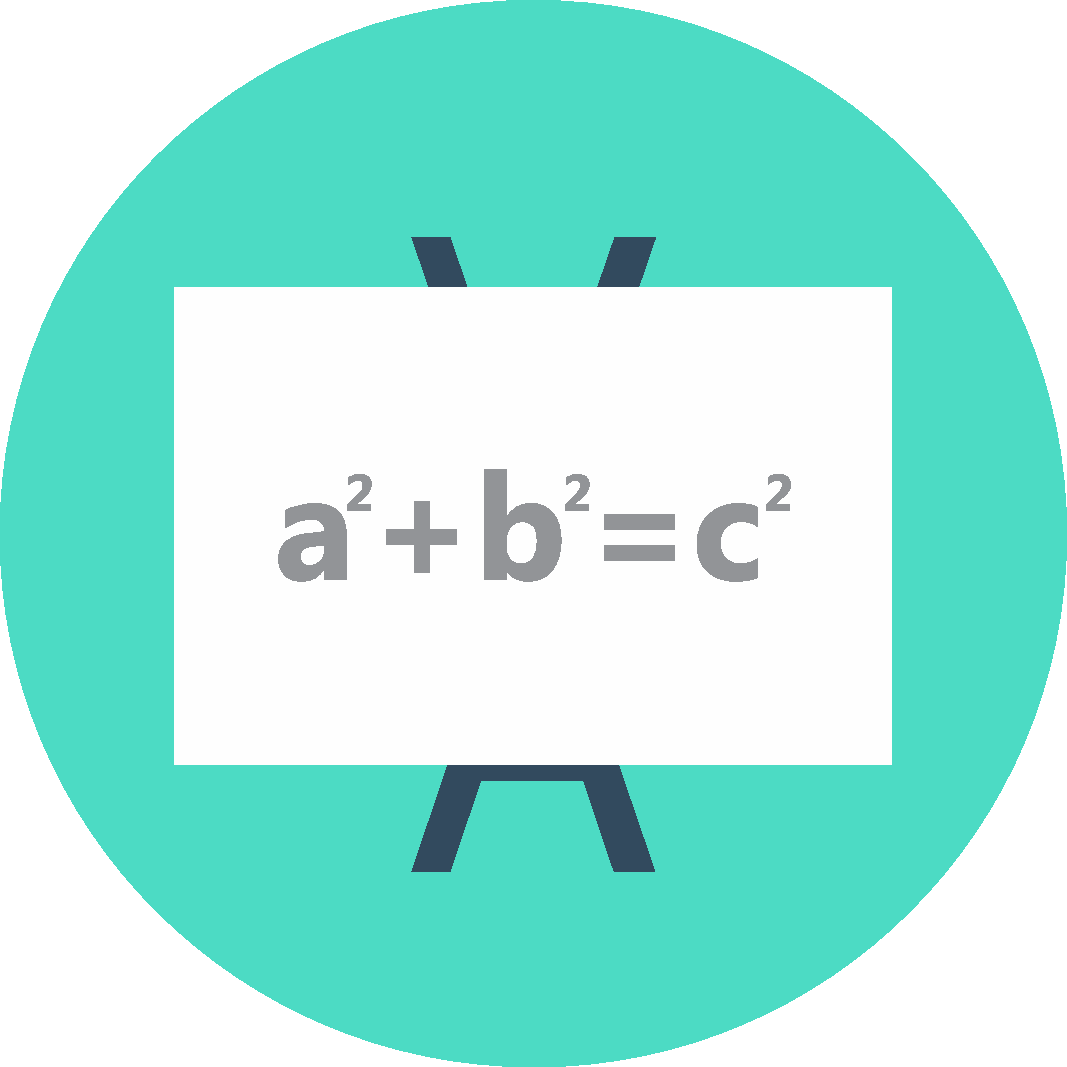
\includegraphics[width=150px]{\imagespath/bacomathiques}%
		
		\vspace{30pt}%
		{\Huge\color{title} #3}%
		
		\vspace{10pt}%
		{Bacomathiques --- \href{https://bacomathiqu.es/cours/#1/#2}{\color{section} https://bacomathiqu.es}}%
		
		\vspace{20pt}%
	\end{center}%
	\begin{toc}
		\tableofcontents%
	\end{toc}
	\thispagestyle{empty}%
	\newpage%
	\setcounter{page}{1}%
}
\newcommand{\imagespath}{../../images}
\newcommand{\lessonimagespath}{\imagespath/lessons/\level/\id/}
\newcommand{\includelatexpicture}[2][\textwidth - 100pt]{%
	\begin{center}%
		\resizebox{#1}{!}{%
			\input{\lessonimagespath#2}%
		}%
	\end{center}%
	\medskip%
}
\newcommand{\includeimage}[1]{%
	\begin{center}%
		\includegraphics{\lessonimagespath#1}%
	\end{center}%
	\medskip%
}
\newcommand{\includerepresentation}[1]{%
	\begin{center}%
		\setlength{\fboxrule}{0.5pt}%
		\href{https://www.geogebra.org/m/#1}{\includegraphics[width=\textwidth-1pt,fbox]{\lessonimagespath#1}}%
	\end{center}%
}
\newcommand{\floor}[1]{\lfloor #1 \rfloor}

\makeatletter
\newcommand\inputcontent{\@ifstar{\inputcontent@star}{\inputcontent@nostar}}
\newcommand{\inputcontent@star}[1]{%
	\ExecuteMetaData[#1]{content}%
}
\newcommand{\inputcontent@nostar}[1]{%
	\newpage%
	\inputcontent@star{#1}%
}
\makeatother

\let\oldsection\section
\renewcommand\section{\clearpage\oldsection}
\newcommand{\contentwidth}[1][medium]{}

% En-têtes :

\pagestyle{fancy}

\renewcommand{\sectionmark}[1]{\markboth{\thesection \ #1}{}}

\fancyhead[R]{\truncate{0.23\textwidth}{\color{title}\thepage}}
\fancyhead[L]{\truncate{0.73\textwidth}{\color{title}\leftmark}}
\fancyfoot[C]{\scriptsize \href{https://bacomathiqu.es/cours/\level/\id}{\texttt{bacomathiqu.es}}}

\makeatletter
\patchcmd{\f@nch@head}{\rlap}{\color{rule}\rlap}{}{}
\patchcmd{\headrule}{\hrule}{\color{rule}\hrule}{}{}
\makeatother

% Environnements :

\newenvironment{nosummary}{}{}
\newcommand{\tcolorboxtitle}[2]{\setlength{\fboxsep}{2.5pt}\hspace{-10pt}\colorbox{#1-left}{\hspace{8pt}\MakeUppercase{#2} \hspace{2pt} \includegraphics[height=0.8em]{\imagespath/bubbles/#1}\hspace{5pt}}}
\newcommand{\tcolorboxsubtitle}[2]{\ifstrempty{#2}{}{\textcolor{#1-left}{\large#2}\\[\medskipamount]}}
\tcbset{
	frame hidden,
	boxrule=0pt,
	boxsep=0pt,
	enlarge bottom by=8.5pt,
	enhanced jigsaw,
	boxed title style={sharp corners,boxrule=0pt,coltitle={white},titlerule=0pt},
	fonttitle=\fontsize{6pt}{6pt}\bfseries\boldmath,
	top=10pt,
	right=10pt,
	bottom=10pt,
	left=10pt,
	arc=0pt,
	outer arc=0pt,
}
\newtcolorbox{toc}[1][]{
	colback=toc,
	borderline west={3pt}{0pt}{toc-left},
	title=\tcolorboxtitle{toc}{Table des matières},
	colbacktitle=toc,
	before upper={\tcolorboxsubtitle{toc}{#1}}
}
\newtcolorbox{formula}[1][]{
	colback=formula,
	borderline west={3pt}{0pt}{formula-left},
	title=\tcolorboxtitle{formula}{À retenir},
	colbacktitle=formula,
	before upper={\tcolorboxsubtitle{formula}{#1}}
}
\newtcolorbox{tip}[1][]{
	colback=tip,
	borderline west={3pt}{0pt}{tip-left},
	title=\tcolorboxtitle{tip}{À lire},
	colbacktitle=tip,
	before upper={\tcolorboxsubtitle{tip}{#1}}
}
\newtcolorbox{demonstration}[1][]{
	colback=demonstration,
	borderline west={3pt}{0pt}{demonstration-left},
	title=\tcolorboxtitle{demonstration}{Démonstration},
	colbacktitle=demonstration,
	before upper={\tcolorboxsubtitle{demonstration}{#1}}
}

\NewEnviron{whitetabularx}[1]{%
	\renewcommand{\arraystretch}{2.5}
	\colorbox{white}{%
		\begin{tabularx}{\textwidth}{#1}%
			\BODY%
		\end{tabularx}%
	}%
}

% Longueurs :

\newlength{\espacetitreliste}
\setlength{\espacetitreliste}{-16pt}
\newcommand{\entretitreetliste}{\vspace{\espacetitreliste}}

\begin{document}
	%<*content>
	\lesson[specialty]{terminale}{16}{chaines-markov}{Chaînes de Markov}

	\header{caption}{On utilise les chaînes de Markov pour étudier et modéliser des réseaux.}

	\header{description}{Une chaîne de Markov est un objet mathématiques qui, couplé à des graphes
		et à des matrices, permet d'étudier un processus aléatoire en fonction du temps.
		Dans ce cours, nous étudierons donc cet objet et ses propriétés, puis nous ferons
		le lien avec les chapitres précédents (via les matrices de transition et les graphes
		probabilistes, notamment). Nous donnerons également quelques exemples de situations
		dans lesquelles on peut appliquer les résultats mathématiques de ce cours.}

	\header{difficulty}{5}

	\section{Graphe pondéré et graphe probabiliste}

	\subsection{Définition}

	\begin{formula}[Graphe pondéré]
		Un graphe est dit \textbf{pondéré} si chacune de ses arêtes est affecté d'un nombre positif (ou nul) que l'on appelle \textbf{poids}.
		\newpar
		Le poids d'une chaîne (ou d'un chemin) est la somme des poids de ses arêtes.
	\end{formula}

	\begin{tip}[Exemple]
		On considère le graphe orienté et pondéré suivant :
		\includelatexpicture{graphe-1}
		On a :
		\begin{itemize}
			\item Le poids de l'arête $A-B$ vaut $0$.
			\item Le poids du chemin $A-B-C-A-D$ vaut $0+4+2+7 = 13$.
		\end{itemize}
	\end{tip}

	\begin{formula}[Graphe probabiliste]
		On appelle \textbf{graphe probabiliste} un graphe orienté et pondéré tel que :
		\begin{itemize}
			\item Pour chaque sommet, la somme des poids des arcs issus de ce sommet vaut $1$.
			\item Il y a au plus $1$ arrête orientée reliant chaque sommet.
		\end{itemize}
	\end{formula}

	Il peut être utile de faire l'analogie entre les graphes probabilistes et \href{https://bacomathiqu.es/cours/premiere/probabilites/#arbre-de-probabilite}{les arbres de probabilité} vus en classe de Première.

	\begin{tip}[Exemple]
		Faisons un exemple concret. On souhaite étudier l'évolution d'une maladie chez un certain individu. À un jour donné, cet individu est soit malade (que l'on note $M$), soit soigné (que l'on note $S$). On suppose que pour cette maladie :
		\begin{itemize}
			\item La probabilité qu'une personne malade guérisse le lendemain est $0,4$.
			\item La probabilité qu'une personne saine tombe malade le lendemain est $0,1$.
		\end{itemize}
		Le graphe probabiliste modélisant cette situation est le graphe $G$ suivant :
		\includelatexpicture{graphe-2}
		On remarque que la somme des poids des arêtes issues du sommet $S$ vaut $0,9+0,1 = 1$ (idem pour $M$ qui vaut $0,6+0,4 = 1$).
	\end{tip}

	\subsection{Matrice de transition}

	\begin{formula}[Définition]
		Soit $G$ un graphe probabiliste d'ordre $n$. On appelle \textbf{matrice de transition} du graphe $G$, la matrice carrée d'ordre $n$ dont le coefficient à la ligne $i$ et à la colonne $j$ est égal au poids de l'arête reliant le sommet $i$ au sommet $j$.
		\newpar
		Une telle matrice est qualifiée de \textbf{stochastique} car la somme des coefficients de chacune de ses lignes vaut $1$.
	\end{formula}

	\begin{tip}[Exemple]
		Dans l'exemple précédent (en supposant que $S$ est le 1\ier{} sommet et que $M$ est le 2\ieme{}) la matrice de transition du graphe $G$ est $\begin{pmatrix} 0,9 & 0,1 \\ 0,4 & 0,6 \end{pmatrix}$.
	\end{tip}

	Attention cependant à ne pas confondre matrice de transition et matrice d'adjacence.

	\section{Chaînes de Markov}

	\subsection{Définition}

	Il vous est fortement conseillé de relire (et de maîtriser) le cours sur \href{https://bacomathiqu.es/cours/terminale/variables-aleatoires-concentration-grands-nombres/}{les variables aléatoires} avant d'aborder cette section. De plus, sachez que cette partie est sans doute la plus difficile du programme de Terminale. Mais ne vous découragez pas car elle reste parfaitement accessible !

	\begin{formula}[Définition]
		Soit $(X_n)$ une suite de variables aléatoires discrètes définies sur un même univers $\Omega$ et à valeurs dans un ensemble $E$. On dit que $(X_n)$ définit une \textbf{chaîne de Markov} sur $E$ si pour tout $n \in \mathbb{N}$ et tout $x_0, x_1, x_2, \dots, x_n \in E$, l'événement $(X_n = x_n)$ ne dépend que de l'événement antérieur $(X_{n-1} = x_{n-1})$ (et pas des précédents) ; autrement dit, si $P_{(X_{n-1} = x_{n-1}) \, \cap \dots \cap \, (X_0 = x_0)}(X_n = x_n) = P_{(X_{n-1} = x_{n-1})}(X_n = x_n)$.
		\newpar
		De plus, l'ensemble $E$ est appelé \textbf{espace des états} de la chaîne de Markov.
	\end{formula}

	En français, cela signifie que si $X_n$ représente l'état d'un système à un temps $n$, alors l'état suivant $X_{n+1}$ ne dépend que de l'état au temps $n$ et pas des états précédents.
	De plus, notez bien que nous n'avons pas fait d'hypothèse sur le cardinal de $E$ (qui peut donc être de cardinal $m \in \mathbb{N}$).
	\begin{nosummary}
		\newpar
		En classe de Terminale, nous nous limiterons principalement au cas où $E$ possède $2$ voire $3$ éléments, mais nous allons quand-même voir très bientôt un exemple de chaîne de Markov à $12$ états.
	\end{nosummary}

	\begin{tip}[Variable aléatoire discrète]
		Une variable aléatoire $X$ définie sur un univers $\Omega$ est dite \textbf{discrète} si $X(\Omega)$ est un ensemble dénombrable.
	\end{tip}

	\begin{formula}[Chaîne de Markov homogène]
		Soit $(X_n)$ une chaîne de Markov dont on note $E$ l'espace des états. Alors $(X_n)$ est dite \textbf{homogène} si pour tout $n \in \mathbb{N}$ et pour tout $x$, $y \in E$, la probabilité $P_{(X_n = x)}(X_{n+1} = y)$ est indépendante de $n$.
		\newpar
		En termes mathématiques, cela signifie que pour tout $n \in \mathbb{N}$ et pour tout $x$, $y \in E$, $P_{(X_n = x)}(X_{n+1} = y) = P_{(X_0 = x)}(X_1 = y)$.
	\end{formula}

	\begin{tip}[Exemple]
		\contentwidth[big]
		Eliott fait la collection des vignettes des 11 joueurs titulaires de l'Équipe de France de football qu'il trouve dans des paquets de céréales. À chaque fois qu'il achète un paquet, il a donc une probabilité de $\frac{1}{11}$ de tomber sur le $k$-ième joueur (pour tout $k$ compris entre $1$ et $11$).
		\newpar
		Si on note par $X_n$ le nombre de vignettes différentes dans la collection d'Eliott après qu'il eut ouvert $n$ paquets de céréales, alors $(X_n)$ est une chaîne de Markov homogène (commençant par $X_0 = 0$). En effet, pour tout $k \in \{0, 1, \dots, 11\}$, on a que l'événement $(X_{n+1} = k)$ ne dépend que de $X_n$ :
		\newpar
		\[ P_A(X_{n+1} = k) = \begin{cases}
      \frac{k}{11} \text{ si } A \text{ est l'événement } (X_n = k) \\
      1 - \frac{k-1}{11} \text{ si } A \text{ est l'événement } (X_n = k-1) \text{ et que } k \geq 1 \\
      0 \text{ sinon}
    \end{cases} \]
		\newpar
		Pour détailler un peu plus :
		\begin{itemize}
			\item Si on a $(X_n = k)$ (i.e. on a déjà tiré $k$ joueurs différents), alors la probabilité d'avoir $(X_{n+1} = k)$ est égale à la probabilité de ne pas tirer de nouveau joueur (qui est $\frac{k}{11}$). Cela inclut également le cas où $k = 11$.
			\item Si on a $(X_n = k-1)$ (i.e. on a déjà tiré $k-1$ joueurs différents), alors la probabilité d'avoir $(X_{n+1} = k)$ est égale à la probabilité de tirer un nouveau joueur (qui est $1 - \frac{k-1}{11}$).
			\item Sinon, comme on ne peut pas tirer plus d'un nouveau joueur d'un coup ou en enlever de la collection, la probabilité d'avoir $(X_{n+1} = k)$ est égale à $0$.
			\item Notons de plus que $(X_n)$ est homogène car le calcul de $P(X_{n+1} = k)$ est indépendant de $n$ (mais reste dépendant de $X_n$, attention).
		\end{itemize}
		De plus, l'espace des états $E$ est $\{0, 1, \dots, 11\}$.
		\newpar
		Cet exemple est très connu et porte un nom : il s'agit du \textbf{problème du collectionneur de vignettes}. Pour votre culture, sachez qu'en moyenne, il faudra ouvrir environ $n \ln(n)$ paquets de céréales pour compléter une collection de $n$ vignettes.
	\end{tip}

	\subsection{Matrice et graphe associés à une chaîne de Markov}

	\begin{formula}[Matrice de transition]
		Soit $(X_n)$ une chaîne de Markov homogène dont on note $E = \{x_1, x_2, \dots, x_m\}$ l'espace des états. La \textbf{matrice de transition} de $(X_n)$ est la matrice carrée d'ordre $m$ dont le coefficient situé à la $i$-ième ligne et à la $j$-ième colonne est égal à $p_{i,j} = P_{(X_n = x_i)}(X_{n+1} = x_j)$.
	\end{formula}

	\begin{tip}
		Comme cette probabilité est indépendante de $n$, on peut tout à fait prendre $n = 0$ dans la définition. On a alors $p_{i,j} = P_{(X_0 = x_i)}(X_1 = x_j)$.
	\end{tip}

	\begin{formula}[Graphe associé à une chaîne de Markov]
		Soit $(X_n)$ une chaîne de Markov homogène dont on note $E = \{x_1, x_2, \dots, x_m\}$ l'espace des états. On associe à cette chaîne de Markov un graphe probabiliste $G$ d'ordre $m$ dont les sommets sont les états $x_i$ et dont les arêtes $x_i - x_j$ sont pondérées par les poids $p_{i,j} = P_{(X_n = x_i)}(X_{n+1} = x_j)$.
		\newpar
		La matrice de transition de $(X_n)$ est égale à la matrice de transition du graphe probabiliste $G$ : il s'agit donc aussi d'une matrice stochastique.
	\end{formula}

	\begin{tip}[Exemple]
		\contentwidth[big]
		Reprenons l'exemple précédent. Alors la matrice de transition associée à $(X_n)$ est la matrice $M \in \mathcal{M}_{12}(\mathbb{R})$ :
		\begingroup
		\renewcommand*{\arraystretch}{1.2}
		\[ M = \begin{pmatrix} 0 & 1 & \dots & 0 & 0 \\ 0 & \frac{1}{11} & \ddots & 0 & 0 \\
		\vdots & \ddots & \ddots & \ddots & \vdots \\ 0 & 0 & \ddots & \frac{10}{11} & \frac{1}{11} \\
		0 & 0 & \dots & 0 & 1 \\ \end{pmatrix} \]
		\endgroup
		Et le graphe associé à $(X_n)$ est le graphe probabiliste d'ordre $12$ :
		\includelatexpicture{graphe-3}
	\end{tip}

	\subsection{Distributions dans une chaîne de Markov}

	\begin{formula}[Proposition]
		Soit $(X_n)$ une chaîne de Markov homogène dont on note $E = \{x_1, x_2, \dots, x_m\}$ l'espace des états. On pose $p_{i,j}^{(k)} = P_{(X_0 = x_i)}(X_k = x_j)$ pour tout $k \in \mathbb{N}^*$ (qui représente la probabilité que la chaîne de Markov $(X_n)$ passe de l'état $x_i$ à l'état $x_j$ en $k$ étapes). On a :
		\[ p_{i,j}^{(k)} = \sum_{q=1}^m p_{i,q}^{(k-1)} \times p_{q,j}^{(1)} = p_{i,1}^{(k-1)} \times p_{1,j}^{(1)} + p_{i,2}^{(k-1)} \times p_{2,j}^{(1)} + \dots + p_{i,m}^{(k-1)} \times p_{m,j}^{(1)} \]
		De plus, comme $(X_n)$ est homogène, $p_{i,j}^{(k)} = p_{i,j}^{(n+k)}$ pour tout $n \in \mathbb{N}$.
	\end{formula}

	\begin{demonstration}[Proposition]
		\contentwidth[big]
		\entretitreetliste
		\begin{align*}
			p_{i,j}^{(k)} &= P_{(X_0 = x_i)}(X_k = x_j) \\
			&= \sum_{q=1}^m P_{(X_0 = x_i)}((X_k = x_j) \, \cap \, (X_{k-1} = x_q)) \\
			&= \sum_{q=1}^m P_{(X_{k-1} = x_q) \, \cap \, (x_0 = x_i)}(X_k = x_j) P_{(X_0 = x_i)}(X_{k-1} = x_q) \text{ (probabilités totales)} \\
			&= \sum_{q=1}^m P_{(X_{k-1} = x_q)}(X_k = x_j) P_{(X_0 = x_i)}(X_{k-1} = x_q) \\
			&= \sum_{q=1}^m P_{(X_0 = x_q)}(X_1 = x_j) P_{(X_0 = x_i)}(X_{k-1} = x_q) \text{ (homogénéité)} \\
			&= \sum_{q=1}^m p_{j,q}^{(1)} \times p_{i,q}^{(k-1)}
		\end{align*}
	\end{demonstration}

	Cette formule semble un petit peu compliquée à interpréter. Elle signifie simplement que la probabilité que la chaîne de Markov $(X_n)$ passe de l'état $x_i$ à l'état $x_j$ en $k$ étapes est égale à la probabilité qu'elle passe de l'état $e_i$ à $e_q$ en une étape, puis de passer de $e_q$ à $e_j$ en $k-1$ étapes. Heureusement, il est possible de la simplifier grandement à l'aide des matrices de transition.

	\begin{formula}[Lien avec la matrice de transition]
		En reprenant les notations précédentes et en notant $M$ la matrice de transition de $(X_n)$, alors $p_{i,j}^{(k)}$ est le coefficient à la ligne $i$ et à la colonne $j$ de la matrice $M^k$.
	\end{formula}

	Enfin, donnons la définition centrale de cette section.

	\begin{formula}[Définition]
		\contentwidth[big]
		Soit $(X_n)$ une chaîne de Markov homogène dont on note $E = \{x_1, x_2, \dots, x_m\}$ l'espace des états. On appelle \textbf{suite des distributions} de $(X_n)$ la suite de matrices $(\pi_n)$, définie pour tout $n \in \mathbb{N}$ par $\pi_n = \begin{pmatrix} P(X_n = x_1) & P(X_n = x_2) & \dots & P(X_n = e_m) \end{pmatrix}$.
		\newpar
		$\pi_n$ est donc une matrice ligne d'ordre $m$ et est appelée \textbf{distribution au temps $n$}.
		\newpar
		$\pi_0$ (la distribution au temps $0$) est appelée \textbf{distribution initiale}.
	\end{formula}

	Une propriété très sympathique des distributions, est que l'on dispose d'une relation de récurrence permettant de calculer facilement la distribution à un temps $n$ donné.

	\begin{formula}[Relation entre $\pi_{n+1}$ et $\pi_n$]
		En reprenant les notations de la définition précédente et en notant $M$ la matrice de transition de $(X_n)$, alors la suite $(\pi_n)$ vérifie une relation de récurrence donnée pour tout $n \in \mathbb{N}$ par $\pi_{n+1} = \pi_n M$.
		\newpar
		On en déduit que pour tout $n \in \mathbb{N}$, $\pi_n = \pi_0 M^n$.
	\end{formula}

	\begin{demonstration}[Relation entre $\pi_{n+1}$ et $\pi_n$]
		\contentwidth[big]
		Soit $n \in \mathbb{N}$. Les événements $(X_n = x_1), (X_n = x_2), \dots, (X_n =x_m)$ partitionnent (recouvrent) notre univers, donc par la formule des probabilités totales appliquée à notre système complet d'événements et à $(X_{n+1} = x_j)$ :
		\begin{align*}
			P(X_{n+1} = x_j) &= P((X_{n+1} = x_j) \, \cap \, (X_n = x_1)) + \dots + P((X_{n+1} = x_j) \, \cap \, (X_n = x_m)) \\
			&= P_{(X_n = x_1)}(X_{n+1} = x_j) \times P(X_n = x_1) + \dots + P_{(X_n = x_m)}(X_{n+1} = x_j) \times (X_n = x_m) \\
			&= \pi_n M
		\end{align*}
		Et la formule $\pi_n = \pi_0 M^n$ se déduit de la formule d'une suite géométrique (où $M$ serait ``la raison'' et $\pi_0$ le premier terme).
	\end{demonstration}

	\begin{tip}[Exemple]
		Intéressons-nous à l'alimentation d'un chat durant la journée. Il dispose de trois gamelles différentes $L$, $C$ et $P$ dans lesquelles se trouvent respectivement du lait, des croquettes et de la pâté.
		On suppose que le chat a commencé sa journée par du lait et que toutes les heures, il se dirige vers une des gamelles suivant le graphe probabiliste ci-dessous :
		\includelatexpicture{graphe-4}
		On note par $X_n$ la variable aléatoire qui donne la gamelle qu'a choisi le chat à la $n$-ième heure. On a donc que $(X_n)$ est une chaîne de Markov homogène dont l'espace des états est $E = \{L; C; P\}$. Si on note $(\pi_n)$ la suite des distributions de $(X_n)$, on a alors que $\pi_0 = \begin{pmatrix} 1 & 0 & 0 \end{pmatrix}$.
		\newpar
		Soit $M$ la matrice de transition $M$ de $(X_n)$. Calculons quelques puissances de $M$ :
		\begin{itemize}
			\item $M = \begin{pmatrix} 0,5 & 0,3 & 0,2 \\ 0,2 & 0,7 & 0,1 \\ 0,3 & 0,3 & 0,4 \end{pmatrix}$
			\item $M^2 = \begin{pmatrix} 0,37 & 0,42 & 0,21 \\ 0,27 & 0,58 & 0,15 \\ 0,33 & 0,42 & 0,25 \end{pmatrix}$
			\item $M^3 = \begin{pmatrix} 0,332 & 0,468 & 0,2 \\ 0,296 & 0,532 & 0,172 \\ 0,324 & 0,468 & 0,208 \end{pmatrix}$
		\end{itemize}
		Ainsi :
		\begin{itemize}
			\item $\pi_1 = \pi_0 M = \begin{pmatrix} 0,5 & 0,3 & 0,2 \end{pmatrix}$
			\item $\pi_2 = \pi_0 M^2 = \begin{pmatrix} 0,37 & 0,42 & 0,21 \end{pmatrix}$
			\item $\pi_3 = \pi_0 M^3 = \begin{pmatrix} 0,332 & 0,468 & 0,2 \end{pmatrix}$
		\end{itemize}
		Et par exemple $p_{1,2}^{(3)} = 0,468$ : la probabilité que le chat passe à sa gamelle de croquettes 3 heures après le lait est d'environ 47 \%.
	\end{tip}

	\subsection{Distribution invariante}

	\begin{formula}[Définition]
		Soit $(X_n)$ une chaîne de Markov homogène de matrice de transition $M$. Une distribution $\pi$ est \textbf{invariante} si les deux conditions suivantes sont respectées :
		\begin{itemize}
			\item $\pi M = \pi$ (donc si $\pi$ est une distribution à un temps $n$, on a $\pi = \pi_n$ et cette condition se résume à avoir $\pi_n = \pi_n M = \pi_{n+1}$).
			\item La somme des coefficients de $\pi$ vaut $1$.
		\end{itemize}
	\end{formula}

	\begin{formula}[Existence et unicité de la distribution invariante au temps $n$]
		Soit $(X_n)$ une chaîne de Markov homogène de matrice de transition $M$.
		\newpar
		Si $M$ ne possède aucun coefficient non nul autre que sur sa diagonale, alors $(X_n)$ admet une unique distribution invariante $\pi$.
	\end{formula}

	\begin{formula}[Convergence de la distribution]
		Soit $(X_n)$ une chaîne de Markov homogène dont on note $(\pi_n)$ la suite des distributions.
		\begin{itemize}
			\item Si $(\pi_n)$ est une suite de matrices convergente, alors elle converge vers une distribution invariante $\pi$.
			\item Si le cardinal de l'ensemble des états de $(X_n)$ est $2$, alors $(\pi_n)$ est convergente (et converge vers la distribution invariante $\pi$).
		\end{itemize}
	\end{formula}

	\begin{tip}[Exemple]
		\contentwidth[big]
		Reprenons l'exemple précédent et voyons si $(X_n)$ admet une distribution invariante.
		\newpar
		Remarquons tout d'abord que la matrice de transition $M$ ne possède aucun coefficient non nul. Donc $(X_n)$ admet une unique distribution invariante $\pi$.
		\newpar
		Posons donc $\pi = \begin{pmatrix} x & y & z \end{pmatrix}$ et déterminons $x$, $y$ et $z$ :
		\newpar
		On doit avoir $\pi M = \pi$. Cela revient à résoudre le système suivant :
		\[ \begin{pmatrix} x & y & z \end{pmatrix} \begin{pmatrix} 0,5 & 0,3 & 0,2 \\ 0,2 & 0,7 & 0,1 \\ 0,3 & 0,3 & 0,4 \end{pmatrix} = \begin{pmatrix} x & y & z \end{pmatrix} \tag{S} \]
		D'où :
		\begin{align*}
			(S) &\iff \begin{pmatrix} 0,5x + 0,2y + 0,3z & 0,3x + 0,7y + 0,3z & 0,2x + 0,1y + 0,4z \end{pmatrix} = \begin{pmatrix} x & y & z \end{pmatrix} \\
			&\iff \begin{cases} \frac{1}{2}x + \frac{1}{5}y + \frac{3}{10}z = x \\ \frac{3}{10}x + \frac{7}{10}y + \frac{3}{10}z = y \\ \frac{1}{5}x + \frac{1}{10}y + \frac{2}{5}z = z \end{cases} \text{ (en passant en écriture fractionnaire)} \\
			&\iff \begin{cases} -\frac{1}{2}x + \frac{1}{5}y + \frac{3}{10}z = 0 \\ \frac{3}{10}x - \frac{3}{10}y + \frac{3}{10}z = 0 \\ \frac{1}{5}x + \frac{1}{10}y - \frac{3}{5}z = 0 \end{cases} \\
			&\iff \begin{cases} x = \frac{2}{5}y + \frac{3}{5}z \\ -\frac{9}{50}y + \frac{12}{25}z = 0 \\ \frac{9}{50}y - \frac{12}{25}z = 0 \end{cases} \\
			&\iff \begin{cases} x = \frac{2}{5} \times \frac{8}{3} z + \frac{3}{5}z = \frac{5}{3}z \\ y = \frac{50}{9} \times \frac{12}{25}z = \frac{8}{3}z \end{cases}
		\end{align*}
		Donc $\pi$ est de la forme $\pi = \begin{pmatrix} \frac{5}{3}z & \frac{8}{3}z & z \end{pmatrix}$. De plus, la somme des coefficients de $\pi$ doit faire $1$, donc :
		\[ \frac{5}{3}z + \frac{8}{3}z + z = 1 \iff \frac{16}{3}z = 1 \iff z = \frac{3}{16} \]
		Donc l'unique distribution invariante $\pi$ de $(X_n)$ est :
		\[ \pi = \begin{pmatrix} \frac{5}{16} & \frac{1}{2} & \frac{3}{16} \end{pmatrix} = \begin{pmatrix} 0,3125 & 0,5 & 0,1875 \end{pmatrix} \]
	\end{tip}
	%</content>
\end{document}
